\begin{corr}{Électrostatique}
\correction{Potentiel de Yukawa}
\begin{enumerate}
	\item L'argument d'une fonction est toujours sans dimension. \fbox{$a$ est donc
	  homogène à une longueur.} Le terme 
	  \begin{equation*}
	  	\dfrac{Q}{4 \pi \epsilon_0 r}
	 \end{equation*}
	  correspond au potentiel électrostatique généré par une charge ponctuelle.
	  On en déduit que \fbox{$Q$ est homogène à une charge.}

  	\item Le champ électrostatique $\vece$ est lié au potentiel $V$ par la
          relation suivante
	  \begin{equation*}
		  \vece = - \grad(V),
	  \end{equation*}
	  qui est vraie en tout point de l'espace. On a alors
	  \begin{equation*}
		  \vece(r) = - \dd{V}{r}(r)\er -\dfrac{1}{r}\dd{V}{\theta}(r)\etheta
		  -\dfrac{1}{r\sin\theta}\dd{V}{\phi}(r)\ephi
		  = \boxed{\dfrac{Q}{4 \pi \epsilon_0 r^2}\exp\left(-\dfrac{r}{a}
		    \right)\left(1 + \dfrac{r}{a}\right)\er}
	  \end{equation*}

  	\item On considère une sphère $\mathcal{S}$ de rayon $r$ et de centre $O$.
	  Cette sphère forme une surface fermée, on peut donc lui appliquer le
	  théorème de Gauss pour connaître la charge $q(r)$ contenue dans cette 
	  dernière
	  \begin{equation*}
		  \oiint_\mathcal{S} \vece(r) \cdot \ds = \dfrac{q(r)}{\epsilon_0}.
	  \end{equation*}
	  Le vecteur surface élémentaire de $\mathcal{S}$ s'écrit
	  \begin{equation*}
		  \ds = r^2 \sin\theta\dtheta\dphi \er.
	  \end{equation*}
	  On a alors
	  \begin{equation*}
		  \vece(r)r^2 \int_0^\pi \sin\theta\dtheta 
		  \int_0^{2\pi} \dphi = \dfrac{q(r)}{\epsilon_0}
		  \iff E(r) \times 4 \pi r^2 = \dfrac{q(r)}{\epsilon_0}
		  \iff \boxed{q(r) = Q\left(1 + \dfrac{r}{a}\right)
			  \exp\left(-\dfrac{r}{a}\right)}
	 \end{equation*}

 	\item \begin{enumerate}
		\item \fbox{$q(r) \underset{r \rightarrow 0}{\rightarrow} Q$}
		\item \fbox{$q(r) \underset{r \rightarrow \infty}{\rightarrow} 0$}
	  \end{enumerate}

	  Cela correspond à une charge ponctuelle $Q$ située en $r = 0$ entouré
	  d'une densité de charge négative dont la charge totale est $-Q$. $a$,
	  qui est la distance de décroissance de l'exponentielle, donne donc \fbox{une taille
	  approximative du nuage électronique} qui entoure le noyau d'un atome.
	  La présence du nuage écrante le potentiel créé par la charge centrale
	  en accélérant sa décroissance.
\end{enumerate}




\correction{Champ gravitationnel dans une cavité}
	\begin{enumerate}
		\item On suppose que la particule est située à l'origine $O$ d'un repère
		sphérique $(O, \er, \etheta, \ephi)$. L'expression des deux champs est alors
		\begin{equation*}
			\vece(P) = \dfrac{q}{4 \pi \epsilon_0 ||OP||^2}\er
			\quad \mathrm{et} \quad \vecg(M) = 
			-\mathcal{G} \dfrac{m}{||OP||^2}\er,
		\end{equation*}
		où $\mathcal{G}$ est la constante universelle de gravitation
		et $\epsilon_0$ la permittivité diélectrique du vide.
		On en déduit l'analogie suivante
		\begin{itemize}
			\item $q \longleftrightarrow m$
			\item $1/4\pi \epsilon_0 \longleftrightarrow -\mathcal{G}$.
		\end{itemize}
	\item On peut alors en déduire un théorème de Gauss pour le champ
		gravitationnel $\vecg$. Soit une surface fermée $\mathcal{S}$,
		contenant une masse $m$, le flux de $\vecg$ à travers cette surface
		est donnée par
	      \begin{equation*}
		      \boxed{\oiint_\mathcal{S} \vecg \cdot \ds = - 4\pi \mathcal{G}m}
	      \end{equation*}
	\item Voir Sec.~\ref{sec:calcul_e}. On a 
	\begin{equation*}
		\boxed{\vecg(M) = g(r) \er.}
	\end{equation*}

\item Voir Sec.~\ref{sec:calcul_e} pour plus de détail. Le théorème de Gauss appliqué
	à une sphère $\mathcal{S}$ de rayon $r$ et de centre $O_1$ donne
	\begin{equation*}
		4 \pi r^2 g(r) =
		\left\{
		\begin{array}{l}
			- 4 \pi \mathcal{G}\times \dfrac{4}{3} \pi r^3 \rho 
			\quad \mathrm{si} \quad r \leq R_1 \\[1em]
			- 4 \pi \mathcal{G} \times \dfrac{4}{3} \pi R_1^3 \rho
			\quad \mathrm{si} \quad r \geq R_1. \\[1em]
		\end{array}
		\right.
	\end{equation*}
	Finalement,
	\begin{equation*}
		\boxed{
		\vecg(M) =
		\left\{
		\begin{array}{l}
			- \dfrac{4\mathcal{G} \pi\rho}{3}  \mitbf{OM}
			\quad \mathrm{si} \quad r \leq R_1 \\[1em]
			- \dfrac{4\mathcal{G} \pi R_1^3}{3||OM||^3}  \mitbf{OM} 
			\quad \mathrm{si} \quad r \geq R_1. \\[1em]
		\end{array}
		\right.
		}
	\end{equation*}

\item Le champ de gravitation $\vecg$ ($\meter \usk \rpsquare \second$)
      est homogène à une accélération.
      La constante universelle de gravitation s'exprime en $
      \cubic \meter \usk \rpsquare \second \usk \reciprocal \kilogram$, la masse volumique
      $\rho$ en $\kilogram \usk \rpcubic \meter$ et $OM$ en $\meter$. Le résultat
      est bien homogène.

      \item En ajoutant cette cavité vide, on perd toutes les symétries et invariances
	    que la distribution de charge présentait. \fbox{L'utilisation du théorème de Gauss
	    est donc peu judicieuse.}

      \item Le modèle de Terre proposé dans l'exercice peut-être obtenue en 
	    additionnant une sphère $S_1$ de masse volumique uniforme $\rho$, de rayon
	    $R_1$ et centrée en $O_1$ et une sphère $\mathcal{S}_1$ de masse volumique
	    uniforme $-\rho$, de rayon $R_2$ et centrée en $O_2$. Le champ de 
	    gravitation $\vecg$ en un point $M$ à l'intérieur de la cavité résulte donc
	    de la superposition des champs générés par les sphères $\mathcal{S}_1$
	    et $\mathcal{S}_2$
	    \begin{equation*}
		    \vecg(M) = \vecg_1(M) + \vecg_2(M) = 
	    -\dfrac{4 \mathcal{G} \pi \rho}{3} (\mitbf{O_1M} - \mitbf{O_2M}) =
	    \boxed{-\dfrac{4 \mathcal{G} \pi \rho}{3} \mitbf{O_1 O_2}}
	    \end{equation*}
	    Le champ est donc uniforme à l'intérieur de la cavité.
	\end{enumerate}


	\correction{Fil chargé}
	Pour cet exercice, il suffit de suivre la recette donnée dans le cours
	(voir Sec.~\ref{sec:calcul_e}).
	\begin{enumerate}
		\item On commence donc bien sûr par réaliser un schéma du système
		  et à choisir un repère adapté aux système, ici un repère
		  cylindrique $(O, \er, \etheta, \ez)$ (voir Fig.~\ref{fig:fil}).
		  Un point de l'espace $M$ est défini par ses coordonnées 
		  $(r, \theta, z)$.
		\item On étudie ensuite les invariances de la distribution de charge
		  qui génère au point $M$ un champ électrostatique
		  \begin{equation*}
			  \vece(M) = E_r(r, \theta, z)\er + E_\theta(r, \theta, z)\etheta +
			             E_z(r, \theta, z)\ez.
		 \end{equation*}
		 \begin{enumerate}
			 \item Le fil est infini, la distribution de charge est
		           donc invariante par translation selon $z$. $\vece$
			   ne dépend pas de $z$.
			 \item Le fil présente une symétrie de révolution.
		           Il est invariant par rotation autour de l'axe $z$.
			   $\vece$ ne dépend donc pas de $\theta$.
		\end{enumerate}
		$\vece$ ne dépend donc que de la distance au fil $r$.

	\item On étudie ensuite les symétries de la distribution de charge.
	\begin{enumerate}
		\item $M$ appartient au plan $(M, \er, \etheta)$ qui est un plan
			de symétrie de la distribution de charge. $\vece(M)$ appartient
		  donc à ce plan.
		\item $M$ appartient au plan $(M, \er, \ez)$ qui est un plan de
		  symétrie de la distribution de charge. $\vece(M)$ appartient 
		  donc à ce plan.
	\end{enumerate}
	$\vece(M)$ doit appartenir aux plans $(M, \er, \etheta)$ et $(M, \er, \ez)$.
	On en déduit que $\vece(M)$ est colinéaire à $\er$.
	\begin{equation*}
		\vece(M) = E_r(r)\er.
	\end{equation*}
	Comme nous avons choisi
	notre point $M$  de manière quelconque, ce résultat est vrai en tout 
	point de l'espace.

	\item On choisit comme surface de Gauss un cylindre de rayon $r$ et de 
	  hauteur $h$ centré sur le fil. Cette surface fermée peut-être vue comme
	  la combinaison de 3 surfaces: la surface latérale du cylindre $\mathcal{S}_l$,
	  le couvercle du cylindre $\mathcal{S}_c$ et le fond du cylindre $\mathcal{S}_f$.
	  L'application du théorème de Gauss à cette surface s'écrit
	  \begin{equation*}
		  \iint_{\mathcal{S}_l} \vece \cdot \ds_l + 
		  \iint_{\mathcal{S}_f} \vece \cdot \ds_f +
	  	  \iint_{\mathcal{S}_c} \vece \cdot \ds_c =
		  \dfrac{\lambda h}{\epsilon_0}
	 \end{equation*}
	 $\ds_f$ et $\ds_c$ sont colinéaires à $\ez$, le produit scalaire
	 entre ces vecteurs surfaciques élémentaires et $\vece$ est donc nul.
	 Finalement, seule la première intégrale nous intéresse. Tous les points 
	 de $\mathcal{S}_l$ ont la même coordonnée radiale. Pour se déplacer sur cette 
	 surface, il suffit de faire varier $\theta$ et $z$. On a donc
	 \begin{equation*}
		 \ds_l = r \dtheta \dz \er.
	\end{equation*}
	Le terme de gauche de l'équation précédente devient donc
	\begin{equation*}
		\iint \vece \cdot \ds_l = E(r)r \int_0^{2\pi}\dtheta \int_0^h\dz
		= E(r) 2\pi rh.
	\end{equation*}
	Finalement, 
	\begin{equation*}
		\boxed{\vece(M) = \dfrac{\lambda}{2 \pi \epsilon_0 r}\er}
	\end{equation*}
\end{enumerate}


\begin{figure}[]
	\centering
	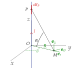
\includegraphics[scale=0.8]{fil}
	\caption{Schéma du fil chargé avec le repère cylindrique associé. 
		La surface de Gauss utilisée apparaît en tiret-pointillé bleu.}%
	\label{fig:fil}
\end{figure}
\end{corr}
